\documentclass[xcolor=dvipsnames,12pt,aspectratio=169]{beamer}
\usecolortheme[named=violet]{structure} 

%\usetheme{umbc2} 
\usepackage{pgf}
%\usepackage[pdftex]{graphicx}
\usepackage{color}
\usepackage{amssymb,amsmath}
\usepackage[english]{babel}
\mode<presentation>

 \usepackage{multimedia}
\usefonttheme{structurebold}

%\useinnertheme{umbcboxes}

%\setbeamercolor{umbcboxes}{bg=violet!15,fg=black}  

\setbeamercovered{transparent}
\setbeamertemplate{navigation symbols}{}
\input{./math-macros}
\setlength{\parskip}{2ex}   % place a blank line between paragraphs
\def\Logo{\@ifnextchar(\beamer@Logo\logo}
\def\beamer@Logo(#1,#2){\logo}

\AtBeginSection[]{
{\setbeamertemplate{logo}{}
 \begin{frame}<beamer>
    \frametitle{Agenda}
    \tableofcontents[currentsection]
  \end{frame}
}
}
% Images
% Macros
\newcommand{\peq}{\,+\hspace{-0.15cm}=}
\newcommand{\bm}{\bar{m}}
\newcommand{\dm}{\delta m}
\newcommand{\dom}{\delta \bar{m}}
\newcommand{\doma}{\delta \bar{m}_{\alpha}}
\newcommand{\om}{\bar{m}}
\newcommand{\bH}{{\bf H}}
\newcommand{\bR}{{\bf R}}
\newcommand{\bcF}{{\bar{\cal F}}}
\newcommand{\cF}{{\cal F}}
\newcommand{\oF}{\bar{F}}
\newcommand{\of}{\bar{f}}
\newcommand{\ou}{\bar{u}}
\newcommand{\odF}{\bar{F}^{\dagger}}
\newcommand{\oS}{\bar{S}}
\newcommand{\oM}{\bar{M}}
\newcommand{\oJa}{\bar{J}_{\alpha}}
\newcommand{\Na}{N_{\alpha}}
\newcommand{\dd}{\delta d}
\newcommand{\ddl}{\delta d_{\alpha}}
\newcommand{\fl}{f_{\lambda}}
\newcommand{\us}{u_{\sigma}}
\newcommand{\pl}{p_{\lambda}}
\newcommand{\dl}{d_{\lambda}}
\newcommand\blfootnote[1]{\begingroup\renewcommand\thefootnote{}\footnote{#1}\addtocounter{footnote}{-1}\endgroup}


\title[]{Approximately Kinematic Waveform Inversion Methods}
\author[]{William W. Symes}
\institute[]{\inst{} Rice University}
\date{SIAM Annual Meeting, 2026}

\begin{document}
\frame{
\titlepage
}

\renewcommand{\thefootnote}{\fnsymbol{footnote}}


\section{Waves \& Rays}
\frame{
  Acoustic waves radiating from isotropic point source
  at $\bx_s \in \bR^3$ with waveform $f(t)$ - solves
  \[
    \square q(\bx,t;\bx_s)  = \left(\frac{1}{\kappa}\frac{\partial^2 q}{\partial t^2} - \frac{1}{\rho}\nabla^2 q\right)(\bx,t;\bx_s)=
    f(t) \delta(\bx-\bx_s),\,q=0 \mbox{ for } t \ll 0
  \]
  $q = $ potential\\
  $\kappa = $ bulk modulus\\
  $\rho = $ density\\
  $f  = $ source time function\\
  $p = \rho \partial_t q = $ pressure
}

\frame{
Waveform data:: emit waves at $\bx_s$, record pressure at $\bx_r$,
Source-receiver pairs $X_{sr} = \{(\bx_s,\bx_r)\}$

Simplify: density $\rho >0$, source waveform $f \in
C_0^{\infty}(\bR)$ {\color{blue} known}; \\also $\log \kappa \in
C^{\infty}(\bR^3) \cap L^{\infty}(\bR^3)$

Predicted pressure data $p[\kappa](\bx_r,t;\bx_s)$

  {\color{blue} Dynamic Inverse Problem}: given data
  $\{d(\bx_r,\cdot;\bx_s): (\bx_s,\bx_r) \in X_{sr}\}$, seek $\kappa$ so that $p[\kappa]
  \approx d$.

  Many variants, large literature since '70's, many apps 
}


\frame{
  High frequency asymptotics (geometric optics/acoustics,...): in
  HF limit, travel time of wave from source at $\bx_s$ to receiver
  at $\bx_r$ is {\em geodesic distance} $\tau[\kappa](\bx_s,\bx_r)$ in metric $ c(\bx)^{-2}\sum_i dx_i
  \otimes dx_i$, $c = \sqrt{\kappa/\rho}$ = sound speed

{\color{blue} Kinematic Inverse Problem:} given times
    $\{t(\bx_s,\bx_r): (\bx_s,\bx_r) \in X_{sr}\}$, find $\kappa$ so
    that $\tau[\kappa] \approx t$

Huge literature - eg. boundary rigidity problem (find $c$ in $\Omega
\subset \bR^n, X_{sr} \subset \partial \Omega$), many apps (seismic
tomography,...)

Complication: multiple geodesics (``rays'') may connect
source/receiver points - which $\tau$ to match?
}


\frame{
  Common computational approach: pose as
  optimization, eg. least squares - use iterative algorithm to find
  $\kappa$ to (approximately) minimize
  \[
  J_{\rm FWI}[\kappa,d] = \sum_{(\bx_s,\bx_r) \in X_{sr}} \int\,dt\,
|p[\kappa](\bx_r,t;\bx_s) - d(\bx_r,t;\bx_s)|^2
\]
(``Full Waveform Inversion'') or
\[
  J_{\rm TTI}[\kappa,t] = \sum_{(\bx_s,\bx_r) \in X_{sr}}
|\tau[\kappa](\bx_s,\bx_r) - t(\bx_s,\bx_r)|^2
\]
(``Travel Time Inversion'')

+ regularizations, constraints
}

%(needs numerics for $\kappa] \rightarrow  p, \tau$ and derivatives
%w.r.t. $\kappa$ - many choices, but often very large scale)

\section{Cycle-skipping}

\frame{
Good news, bad news...

For FWI,
\begin{itemize}
\item seismology, ultrasonic imaging, ocean acoustics,... the
  data are pressure (or acceleration, or stress, or ...), so FWI is the natural
  approach, BUT...
\item local optimization
  (eg. quasi-Newton), required because frequency range $\Rightarrow$ fine discretization $\Rightarrow$ large
  problem size, BUT  unless initial $\kappa$ is kinematically accurate 
  (predicts traveltimes ``within a half-wavelength''), local
  optimization tends to
  stagnate at incorrect final $\kappa$ with big data prediction
  error - worse for higher frequency data  (``cycle-skipping'')
\end{itemize}

}

\frame{
\begin{center}
  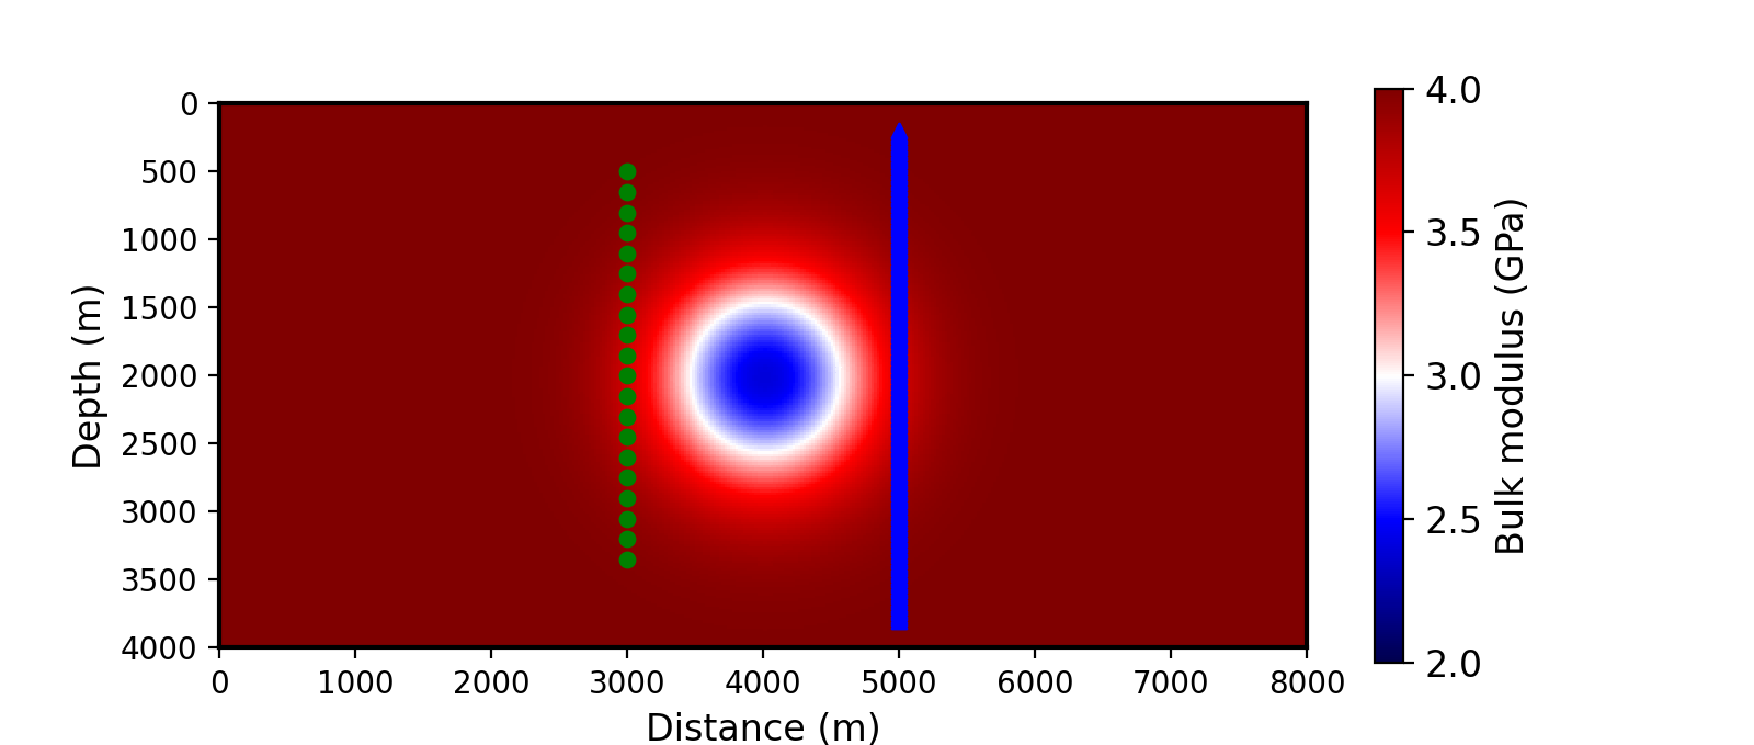
\includegraphics[width=0.45\textwidth]{m}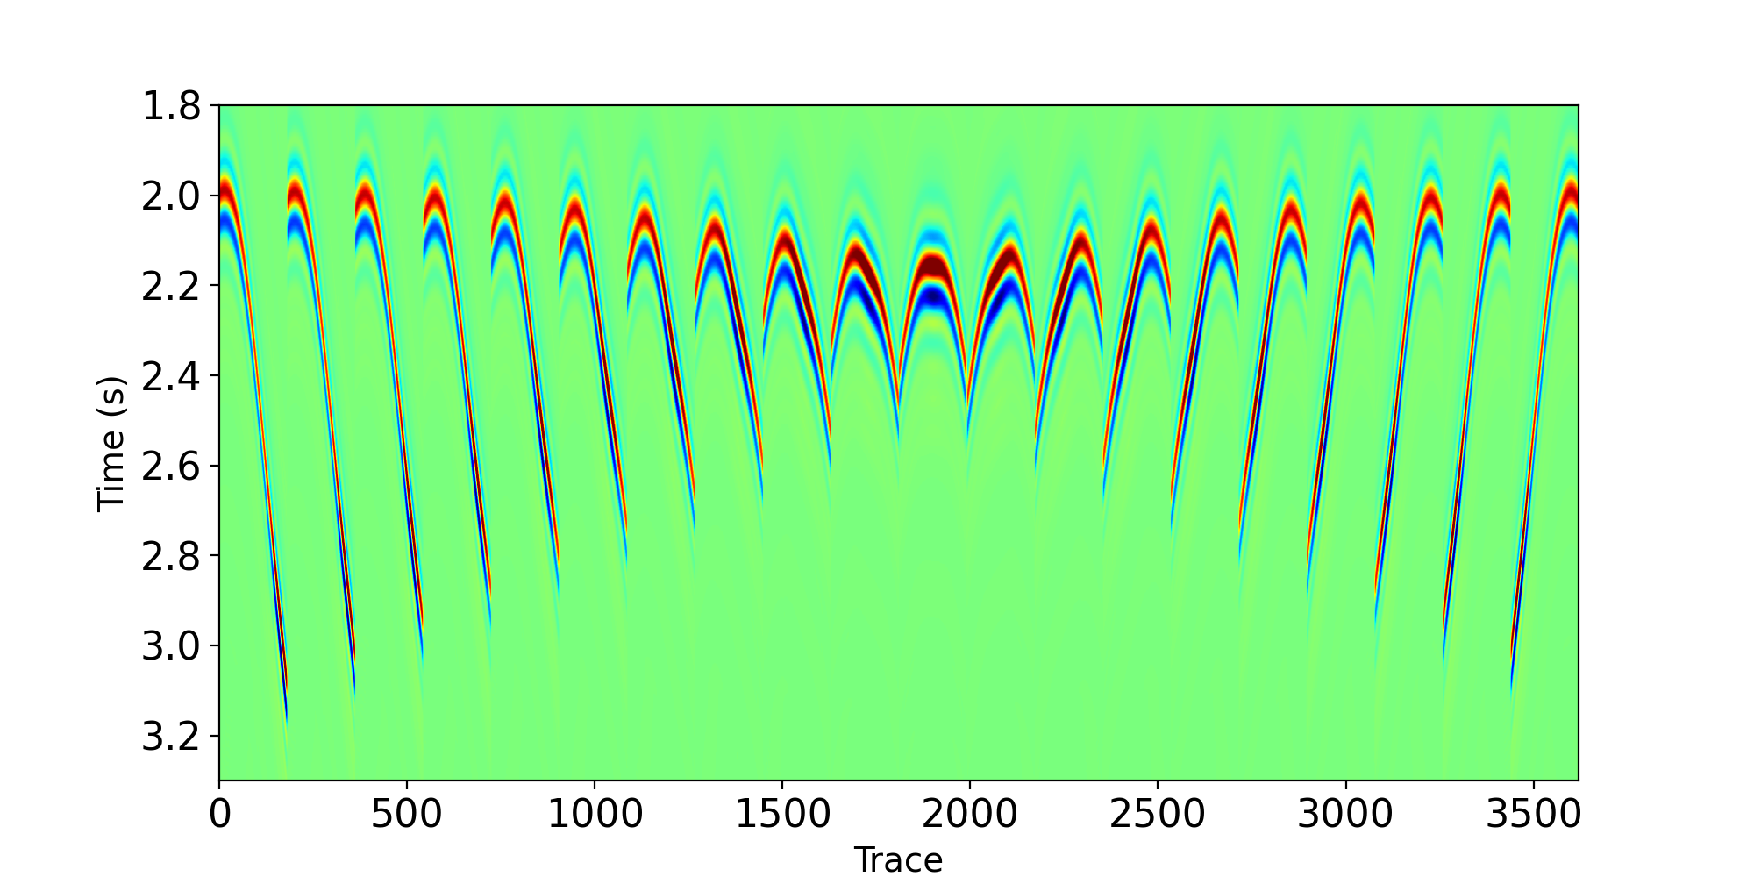
\includegraphics[width=0.40\textwidth]{cwd20}
\end{center}

Left: 2D bulk modulus field (``lens'') $\kappa^*$, 20 source positions ($\bx_s=(x_s,z_s)$, green) at
$x_s=3000$ m, 181 receiver positions ($\bx_r=(x_r,z_r)$, blue) at
$x_r=5000$ m.

Right:
predicted data $d^*(\bx_r,t;\bx_s)=p[\kappa^*](\bx_r,t;\bx_s)$. Time
increases downwards; histories for each $z_s$ grouped together in
order of increasing $z_r$. Note sag in middle.

(from S., Chen \& Minkoff, {\em Inverse
Problems} 41 (6), 2025)
}

\frame{
\begin{center}
  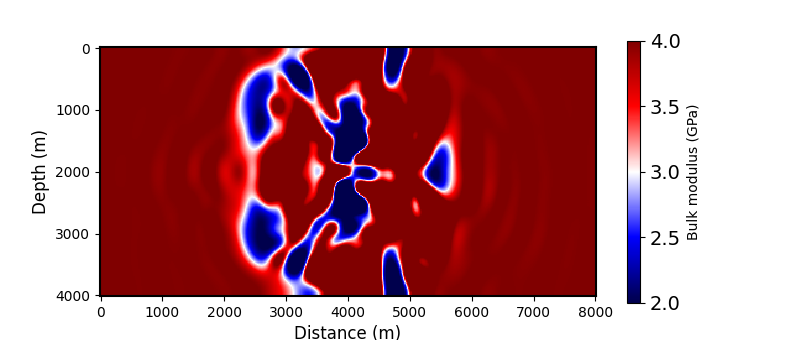
\includegraphics[width=0.45\textwidth]{mestfwi0_200iter}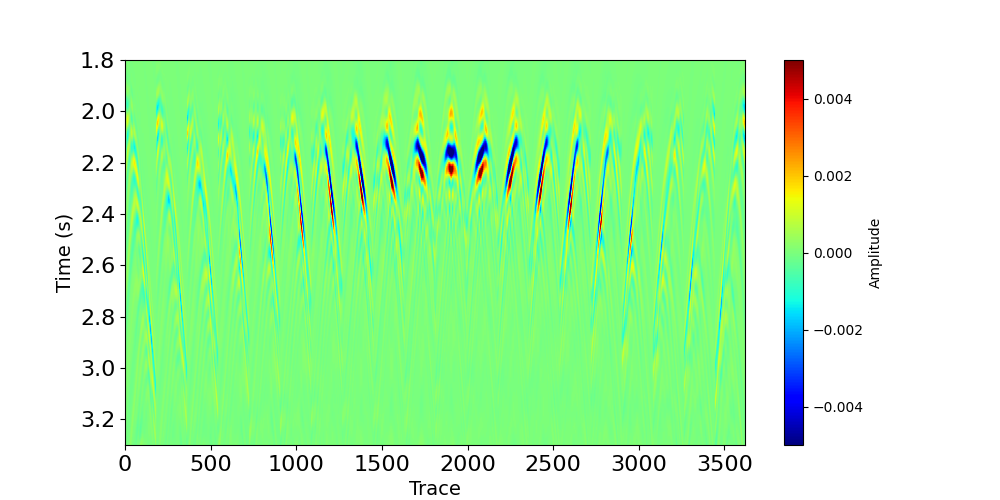
\includegraphics[width=0.40\textwidth]{residmestfwi0_200iter}
\end{center}
  Cycle-skipping in action. Left: Estimated $\kappa_{200}$ from 200 LBFGS iterations on
  $J_{\rm FWI}$, from initial estimate $\kappa_0 \equiv$ 4.0 GPa,
  using data $d$ from ``lens'' $\kappa$. Right: residual
  $p[\kappa_{200}] - d$. RMS relative error = 0.43.
}

\frame{

For TTI,
\begin{itemize}
\item $J_{TTI}$ {\em a priori} unrelated to wavelength, local optimizations tend to
  converge to good fit, BUT...
\item data t are not directly measured, must be inferred
  (``picked'') from waveform data - mostly automated in
  industrial codes, but can be noise-sensitive
\end{itemize}

Conventional remedy for cycle skipping: TTI followed by FWI. Pick times
$t(\bx_r,\bx_s)$, minimize $J_{\rm TTI}$, initiate minimization of
$J_{\rm FWI}$ from result, low $\rightarrow$ high frequency
continuation - widespread use, much success (including commercial)

Q: is there a replacement for FWI
that uses waveform data directly but implicitly
does TTI (so no cycle-skip) - that is, 
{\color{blue} approximately kinematic}?
}


\section{Adaptive Waveform Inversion}

\frame{
  A: yes, at least sometimes...
  
Warner et al. (2012, ...): FWI fails because initial predicted
data $p[k]$ places waves at wrong times $\Rightarrow$ big error - so
{\em move them} to make error small

Use a {\em filter} (convolution kernel) $u_{\sigma}[\kappa,d](\bx_r,t;\bx_s)$, solution of
\[
  \us[\kappa,d] = \mbox{argmin}_u (\|p[\kappa] * u - d\|^2 + \sigma \|u\|^2)
\]
regularization weight $\sigma > 0$ TBD so that $p[\kappa]*u \approx d$

($*$ = convolution in $t$, $\|\cdot\| = L^2$ norm)
}

\frame{
  \begin{center}
    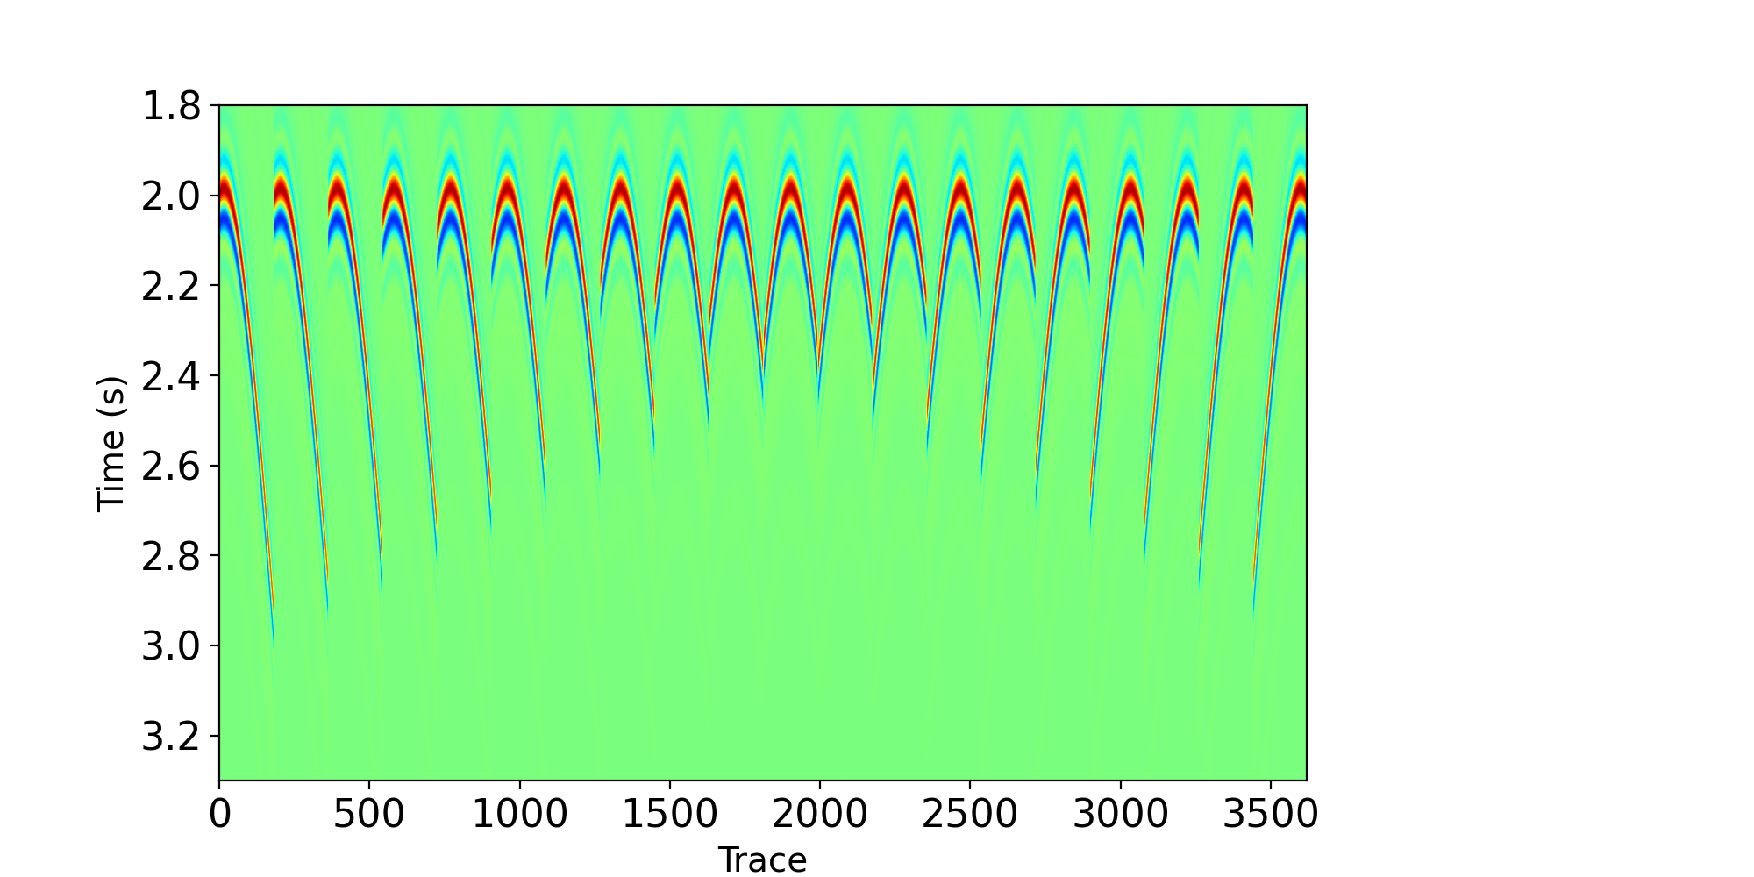
\includegraphics[width=0.4\textwidth,height=2.8cm]{chwd20crop}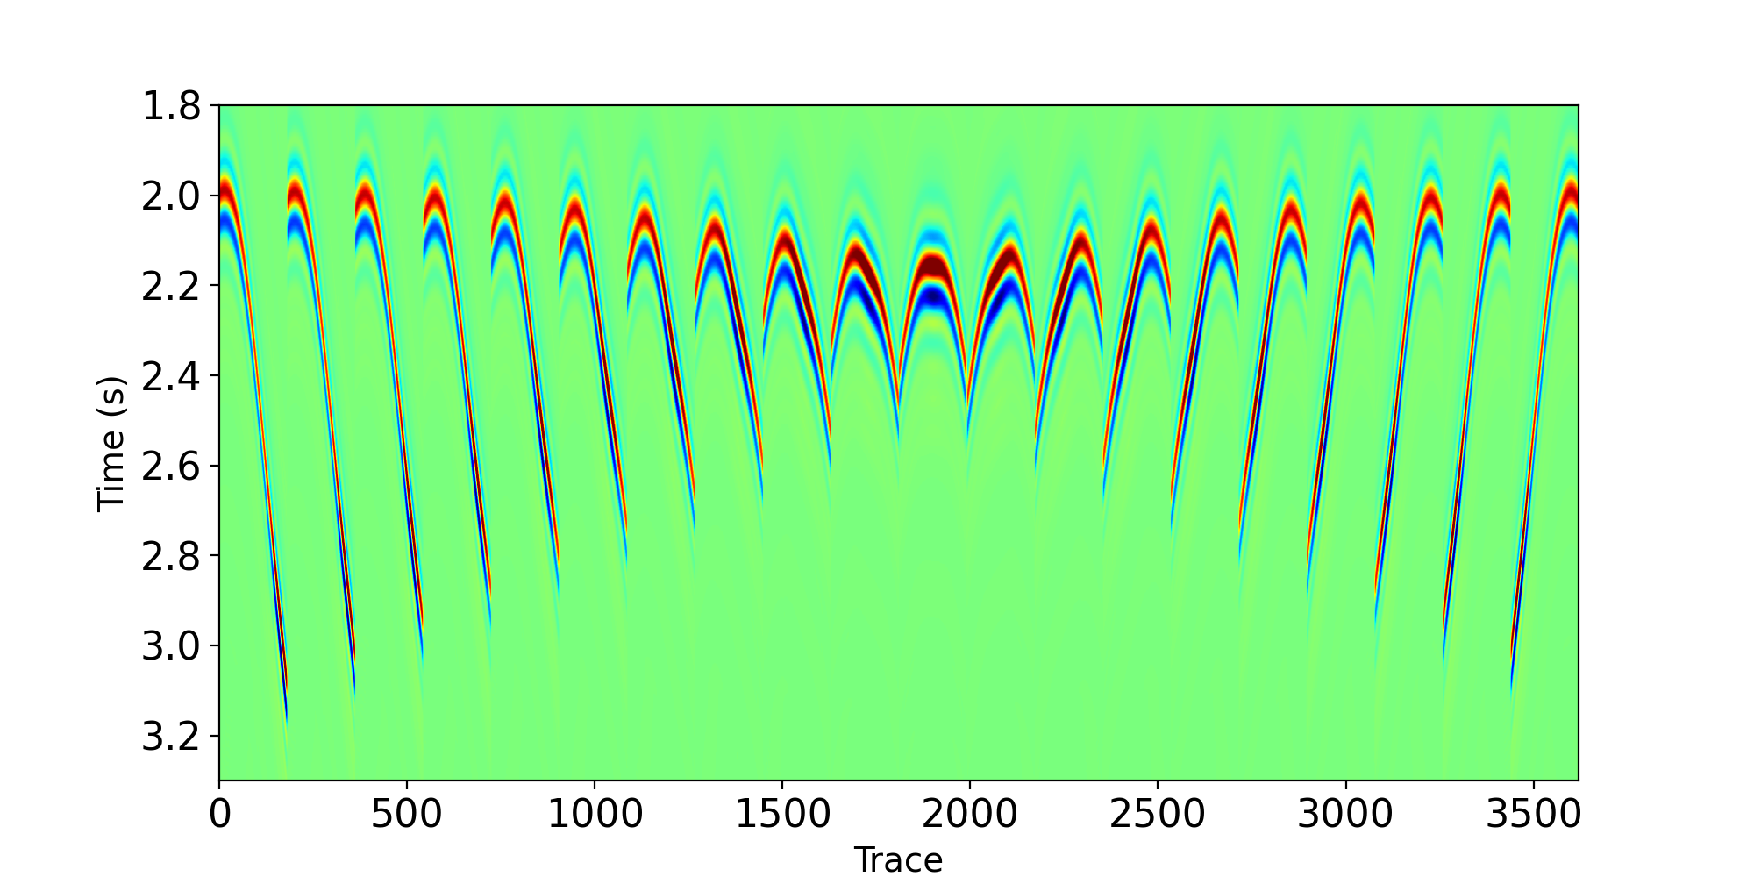
\includegraphics[width=0.40\textwidth]{cwd20}\\
    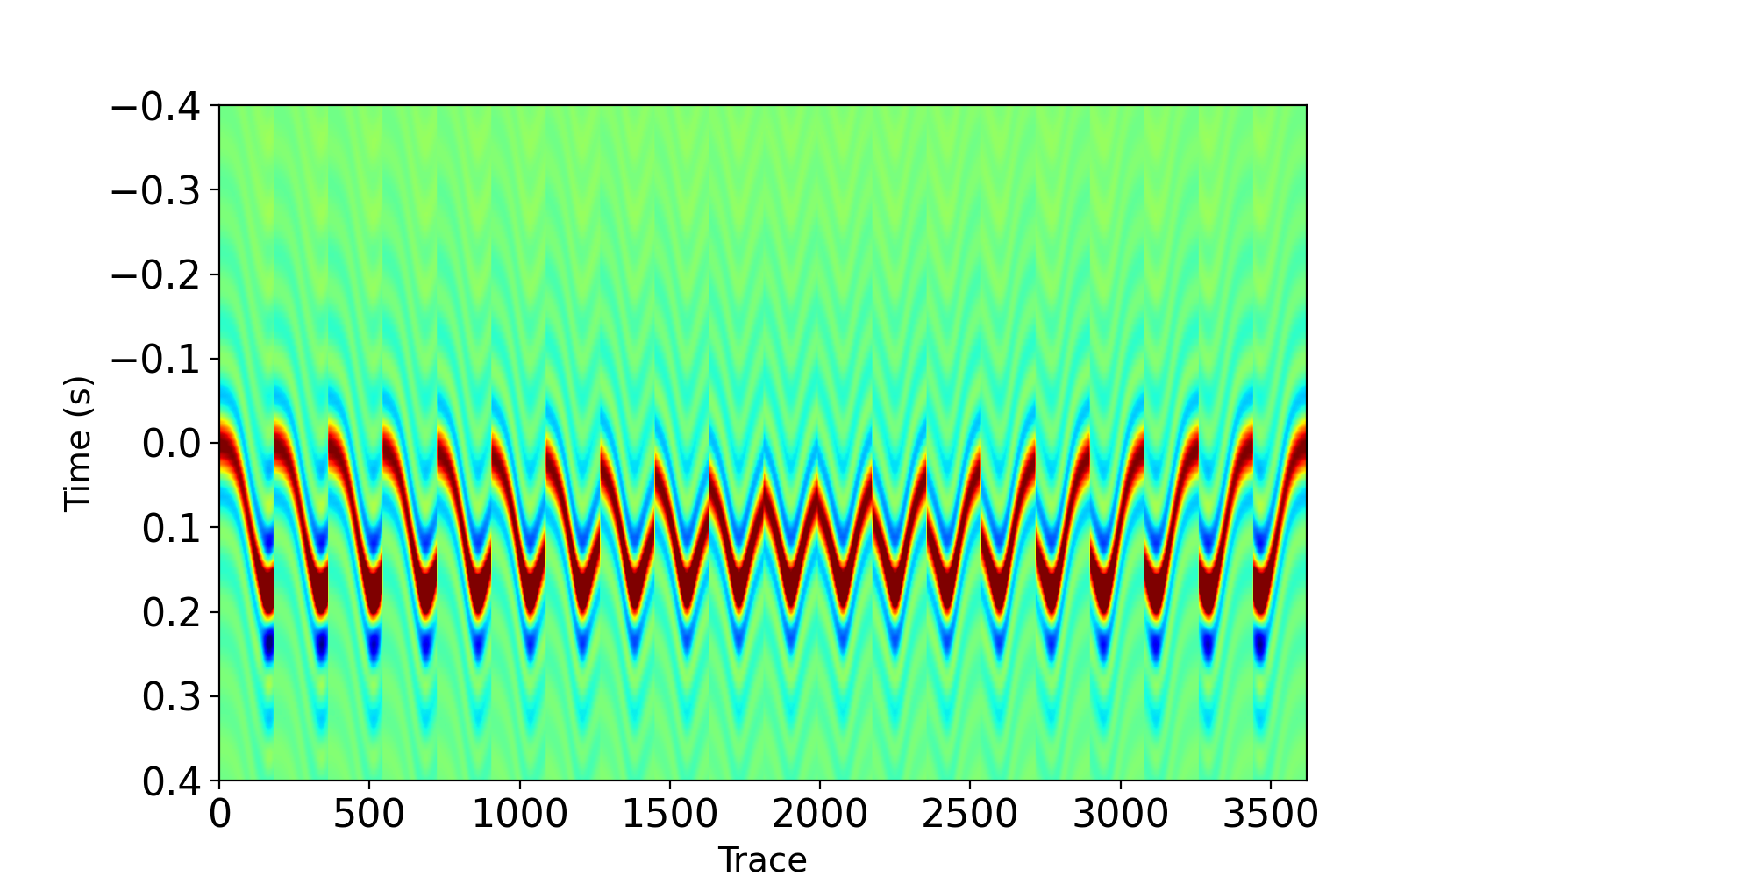
\includegraphics[width=0.4\textwidth,height=2.8cm]{cwlens20uest0crop}
  \end{center}
  Top Left: $p[\kappa_0], \kappa_0\equiv 4.0$ GPa. Top Right: target
  data $d^*=p[\kappa^*]$. Bottom: filter $\us[\kappa_0,d]$, achieves
  $p[\kappa_0]*\us \approx d^*$ (least squares, via CG iteration)
}

\frame{
  BUT want $p[\kappa] \approx d$, not $p[\kappa]*u
  \approx d$ - these are same if $u = \delta(t)$

  {\color{blue} Adaptive Waveform Inversion} (AWI): Since $t\delta(t) =0$,
  try minimizing (over $\kappa$)
  \[
    J_{{\rm AWI},\sigma}[\kappa,d] = \sum_{(\bx_r,\bx_s) \in X_{sr}} \frac{\|tu_{\sigma}[\kappa,d](\bx_r,\cdot;\bx_s)\|^2}{\|u_{\sigma}[\kappa,d](\bx_r,\cdot;\bx_s)\|^2}
  \]
  
  Many successful results reported - overcomes cycle skipping! (at
  least sometimes...) 

  Q: Why should this work? 

  
}

\frame{
  A: Under some conditions $ J_{{\rm AWI},\sigma}[\kappa,d]
  \rightarrow J_{TTI}[\kappa,t]$ as data wavelength $\rightarrow 0$ \\
{\color{blue} $\Rightarrow$ AWI is (sometimes) approximately
  (asymptotically) kinematic}

  Assume:

  {\color{blue} only one geodesic connects points near sources and
    receivers (simple metric);}

  once a geodesic leaves neighborhood of $X_{sr}$, it never returns;

  exponential time decay of solutions (eg. non-trapping metric,
  Vainberg '75);

  noise-free data: $d^* = p[\kappa^*]$.

  express asymptotics via family of source waveforms $\{\fl(t) =
  \sqrt{\lambda}f_1(t/\lambda)\}$, $f_1 \in \partial_t^2 C_0^{\infty}(\bR)$,
  corresponding pressures $\pl[\kappa]$.
}

\frame{
  Then:

  (1)  $\us[\kappa,d^*], t\us[\kappa,d^*] \in L^2(\bR \times X_{sr})$, so
  $J_{\rm AWI,\sigma}[\kappa,d^*]$ is well-defined

  (2) $\|\pl[\kappa]*\us[\kappa,\dl^*]-\dl^*\| \ll \|\dl^*\|
  \Leftrightarrow  \sigma \approx  \mbox{ const. } \times \lambda$
 
  (3) $\sigma\propto \lambda$ $\Rightarrow$
  \[
    |J_{\rm AWI,\sigma}[\kappa,\dl^*] - J_{\rm TTI}(\kappa,t^*)| = O(\lambda^2)
  \]
  ($t^*(\bx_s,\bx_r) = \tau[\kappa^*](\bx_s,\bx_r)$)
}

\frame{
  Sketch of proof: 
  Hadamard expansion\footnote{Hadamard 1923, Courant \& Hilbert '62,
    Friedlander '75, H\"{o}rmander '85, Wei et al. '24} of 3D Green's
  function $\Rightarrow$ 
  \[
    p[\kappa](\bx,t;\bx_s) = \rho a[\kappa](\bx.\bx_s)\partial_t f(t-\tau[\kappa](\bx,\bx_s)) +
    \int_{\tau(\bx,\bx_s)}^t ds\,b[\kappa](\bx,s;\bx_s)\partial_t f(t-s)
  \] 
  Solve LS problem for $\us$ by FT: 
\[
    \us[\kappa,d^*]=
    \frac{a[\kappa^*]}{a[\kappa]}g_{\sigma}[\kappa](t-(\tau[\kappa]-\tau[\kappa^*]))
    + ...,\, \hat{g}_{\sigma}[\kappa](\omega) =
    \frac{\rho^2 a[\kappa]^2 \omega^2|\hat{f}(\omega)|^2}{\rho^2 a[\kappa]^2
      \omega^2|\hat{f}(\omega)|^2 + \sigma}
  \]
  whence
\[
    J_{\rm AWI,\sigma}[\kappa,d^*] =\sum_{(\bx_r,\bx_s)\in X_{sr}}\left(
    (\tau[\kappa]-\tau[\kappa]^*)^2 + \frac{\|tg_{\sigma}[\kappa]\|^2}{\|g_{\sigma}[\kappa]\|^2}
  \right) + ...
  \]
}

\frame{
  Asymptotics: $f = \fl$ and $\sigma \propto \lambda$ then
  \[
    = \|\tau[\kappa]-\tau[\kappa^*]\|^2 + O(\lambda^2) + ...
  \]
$O(\lambda^2)$ estimates for ``...'', other fine print - S. '24
  (arXiv) (related: Song '94)
  \begin{center}
    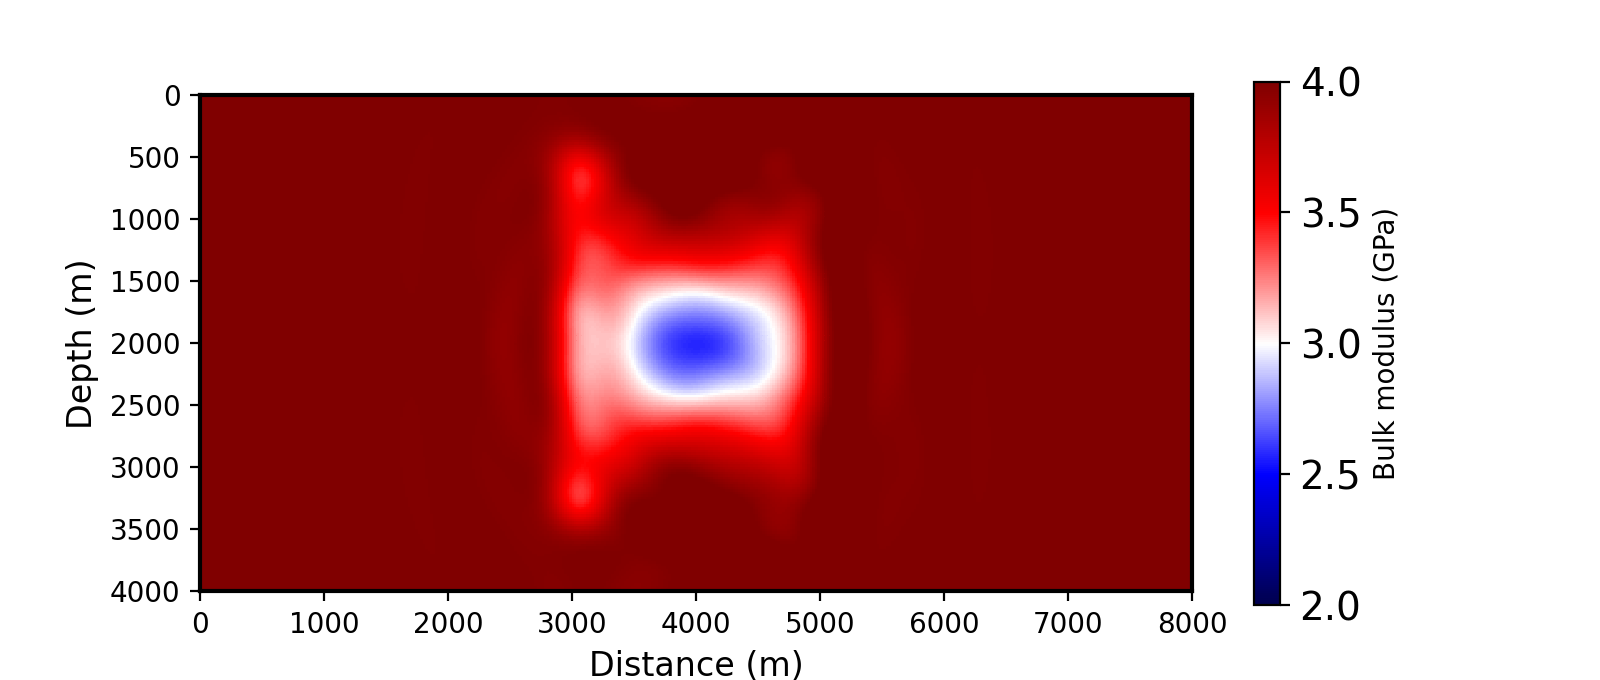
\includegraphics[width=0.45\textwidth]{cwlens20mestmswifwi}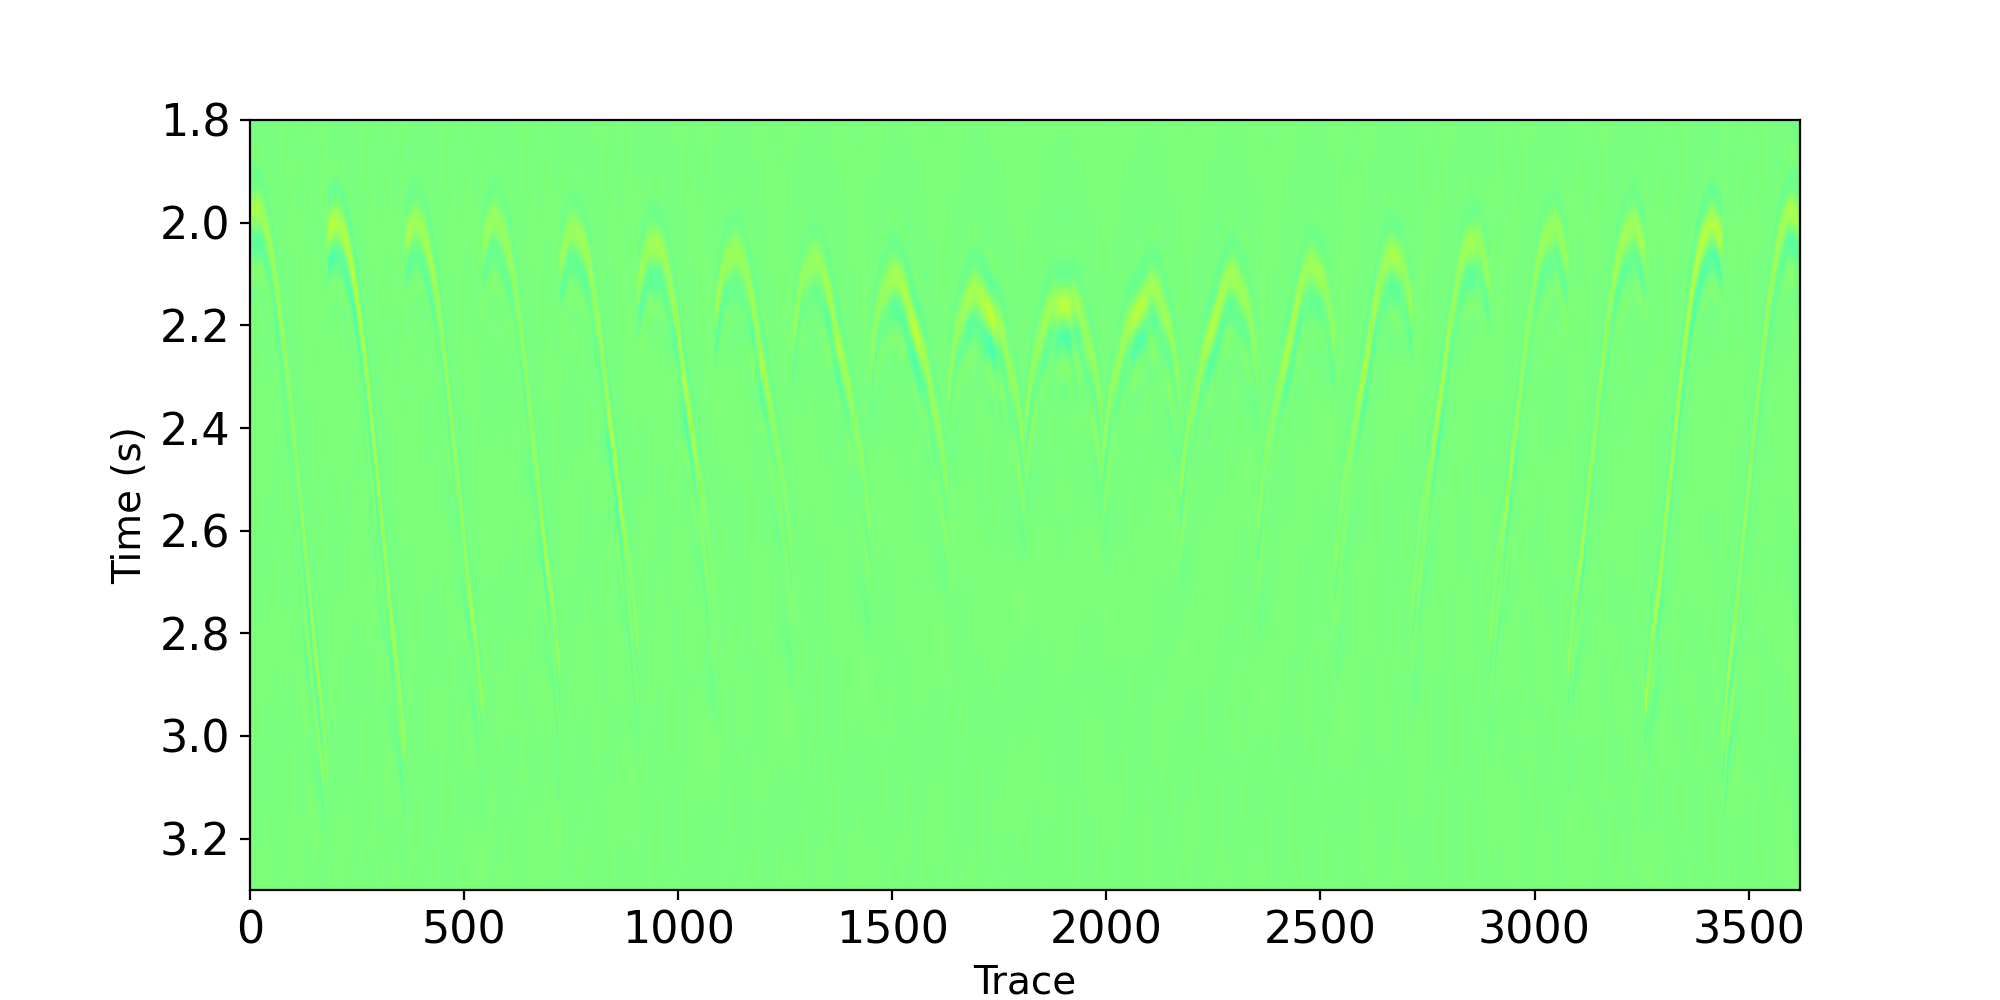
\includegraphics[width=0.40\textwidth]{cwlens20residmestmswifwi}
  \end{center}
  MSWI (= AWI w/o denominator, just $\|t\us\|^2$, similar local
  asymptotics) + FWI: 12 LBFGS iterations each. Left: final estimate
  of $\kappa$. Right: final residual, plotted on same scale as data,
  7\% RMS error.
}

\frame{
  \begin{center}
    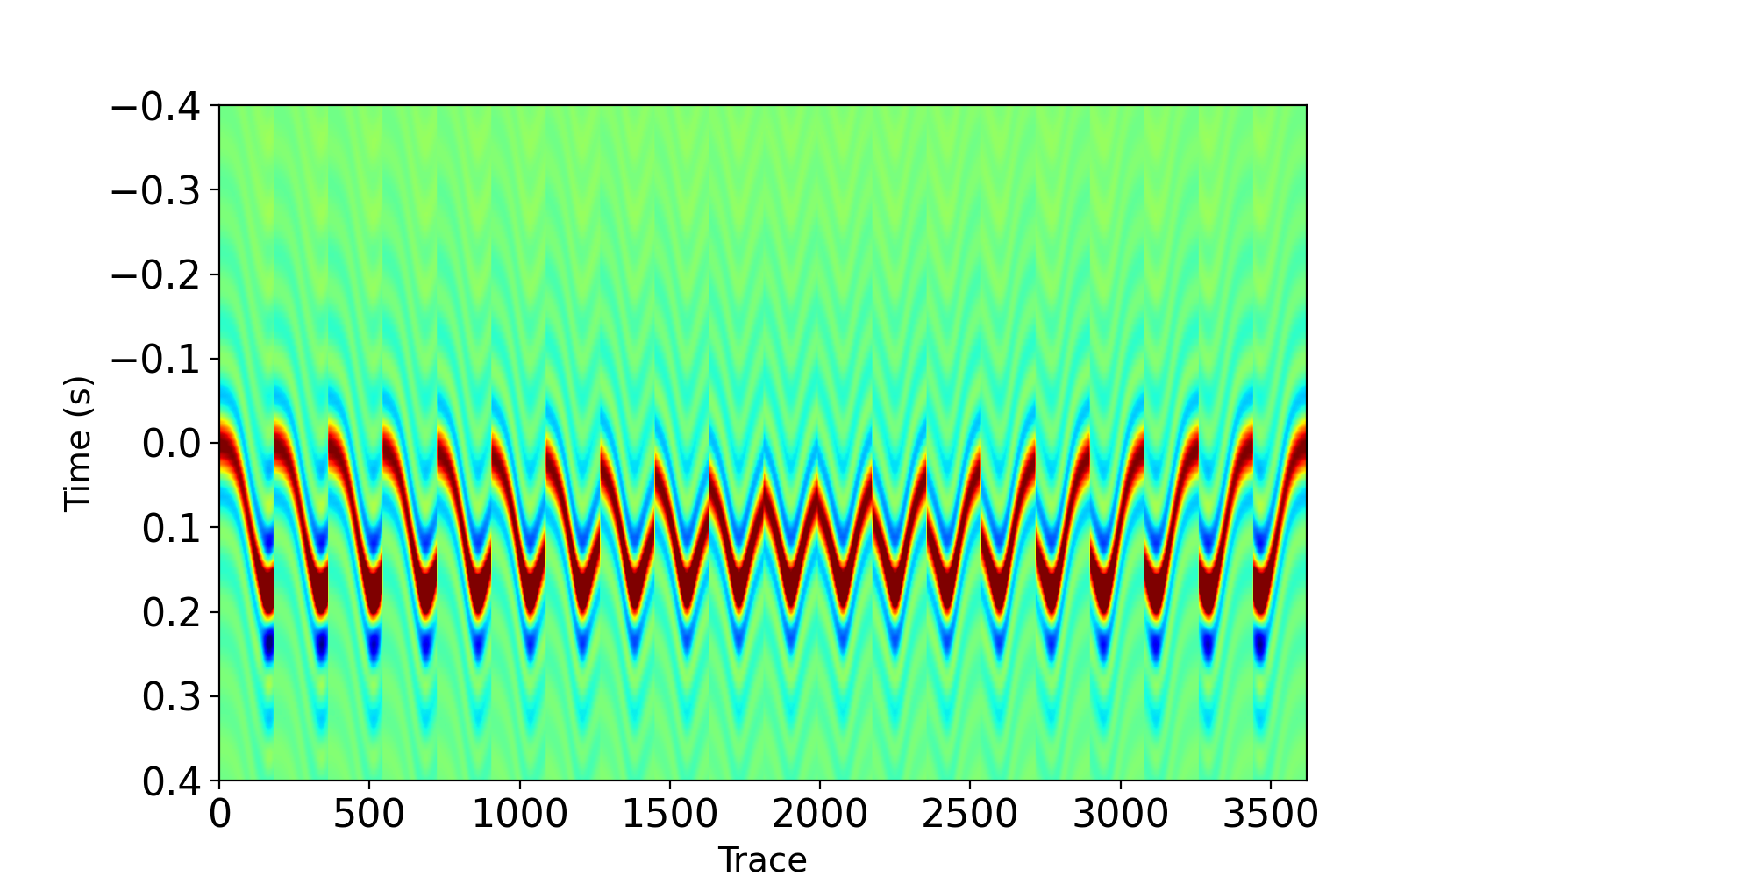
\includegraphics[width=0.40\textwidth,height=2.8cm]{cwlens20uest0crop}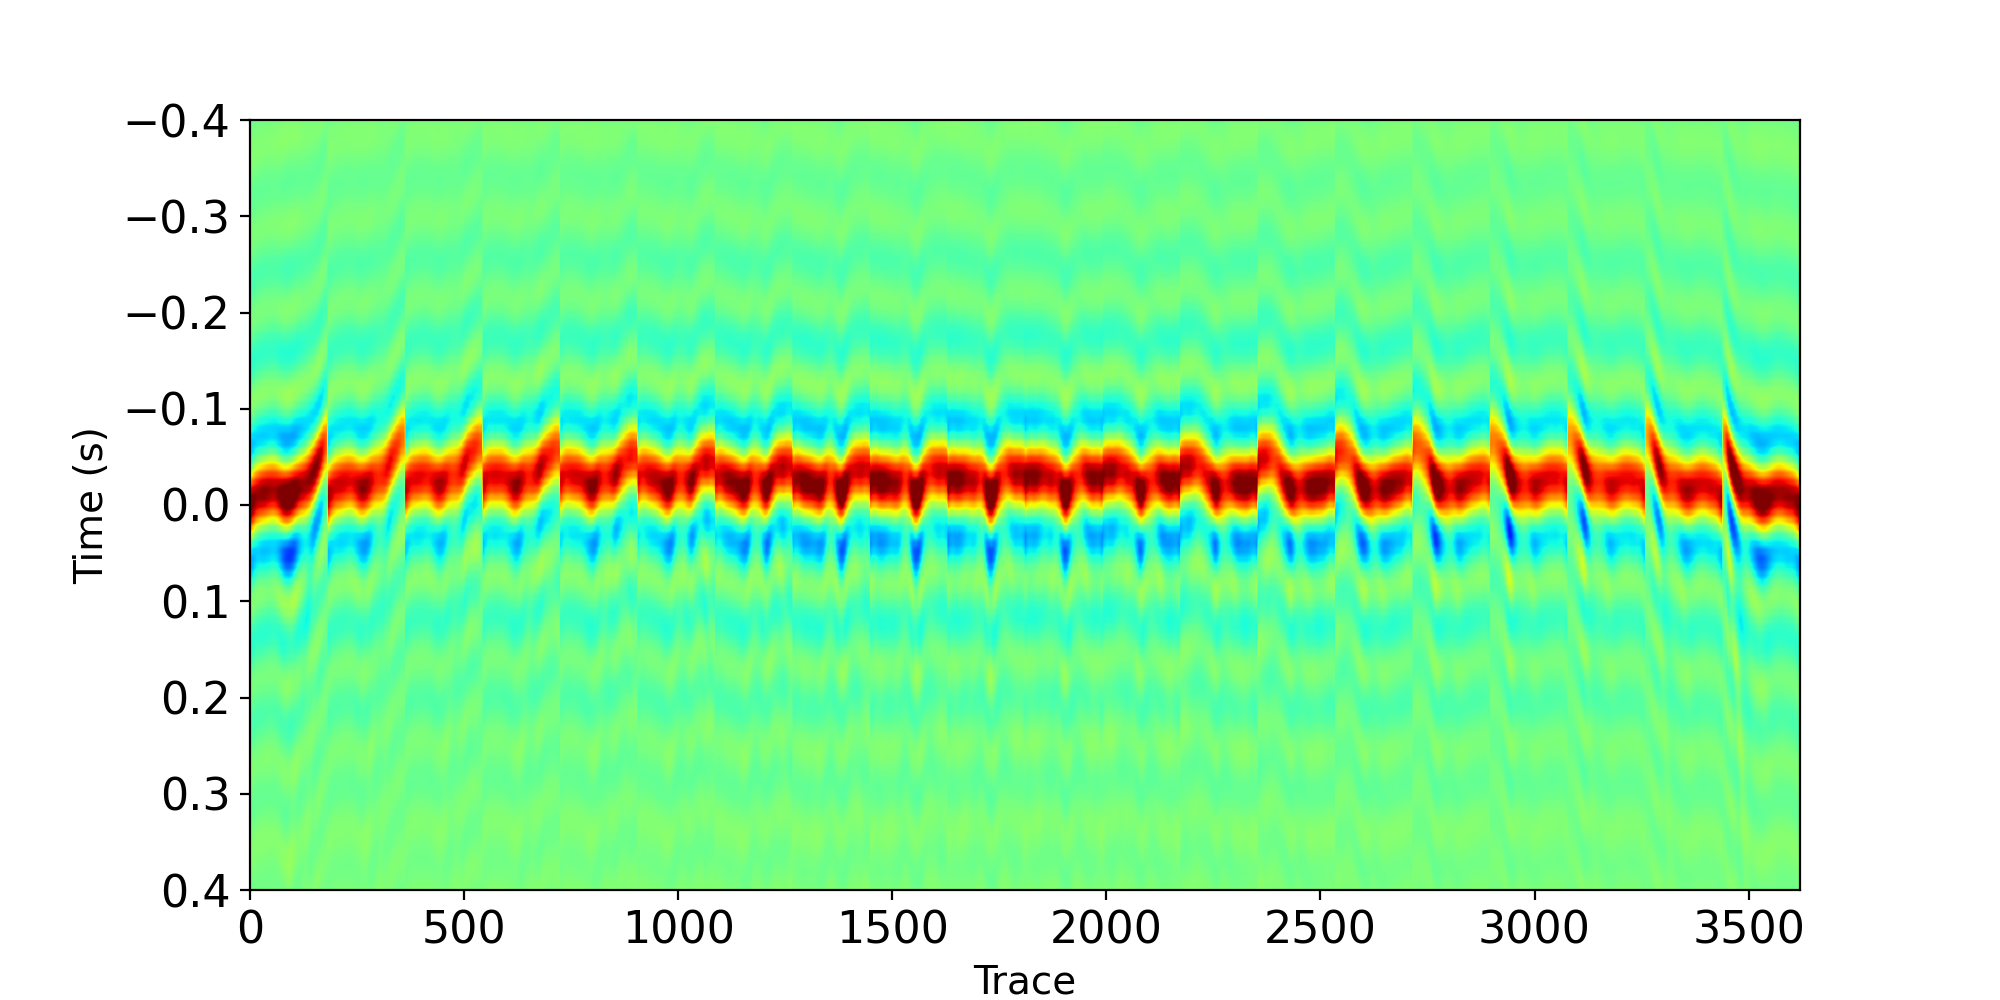
\includegraphics[width=0.40\textwidth]{cwlens20uestmswi}
  \end{center}
  Filter $\us$. Left: at initial estimate $\kappa \equiv 4.0 GPa$.
  Right: at MSWI estimate of $\kappa$, 12 LBFGS iterations (initial
  estimate for FWI).
}

\section{Not done yet...}

\frame{
  Metric not simple (multiple geodesics connect source, receiver
  positions) $\Rightarrow$ asymptotic relation AWI $\leftrightarrow$
  TTI {\color{blue} fails}, AWI cycle skips.

  Why: Interference between multiple wavefronts (S. '94, Huang '19,
  Pladys  '21, Yong '23, S. '24).

  Approximately kinematic modifications of AWI::
  \begin{itemize}
  \item Separate wavefronts in time via Gabor transform: Local AWI (Yong '23)
  \item Separate wavefronts in phase space via spatially extended
    sources (``acoustic antennae''), penalize spatial dispersion
    (Huang '19, S. '23) - asymptotic to non-standard traveltime misfit
    ($\sim$ lens rigidity)
  \end{itemize}
  
  Completely untouched but extremely important: elasticity, EM,
  reflection (non-smooth coefficients), {\color{blue} attenuation}
}

\frame{
  Thanks to
  \begin{itemize}
  \item Hua Song, Guanghui Huang
  \item Huiyi Chen, Sue Minkoff
  \item Profs. Qian and Leung
  \end{itemize}
}
\end{document}
  
\frame{
  Metric not simple (multiple geodesics connect source, receiver
  positions) $\Rightarrow$ asymptotic relation AWI $\leftrightarrow$
  TTI {\color{blue} fails}
  \begin{center}
    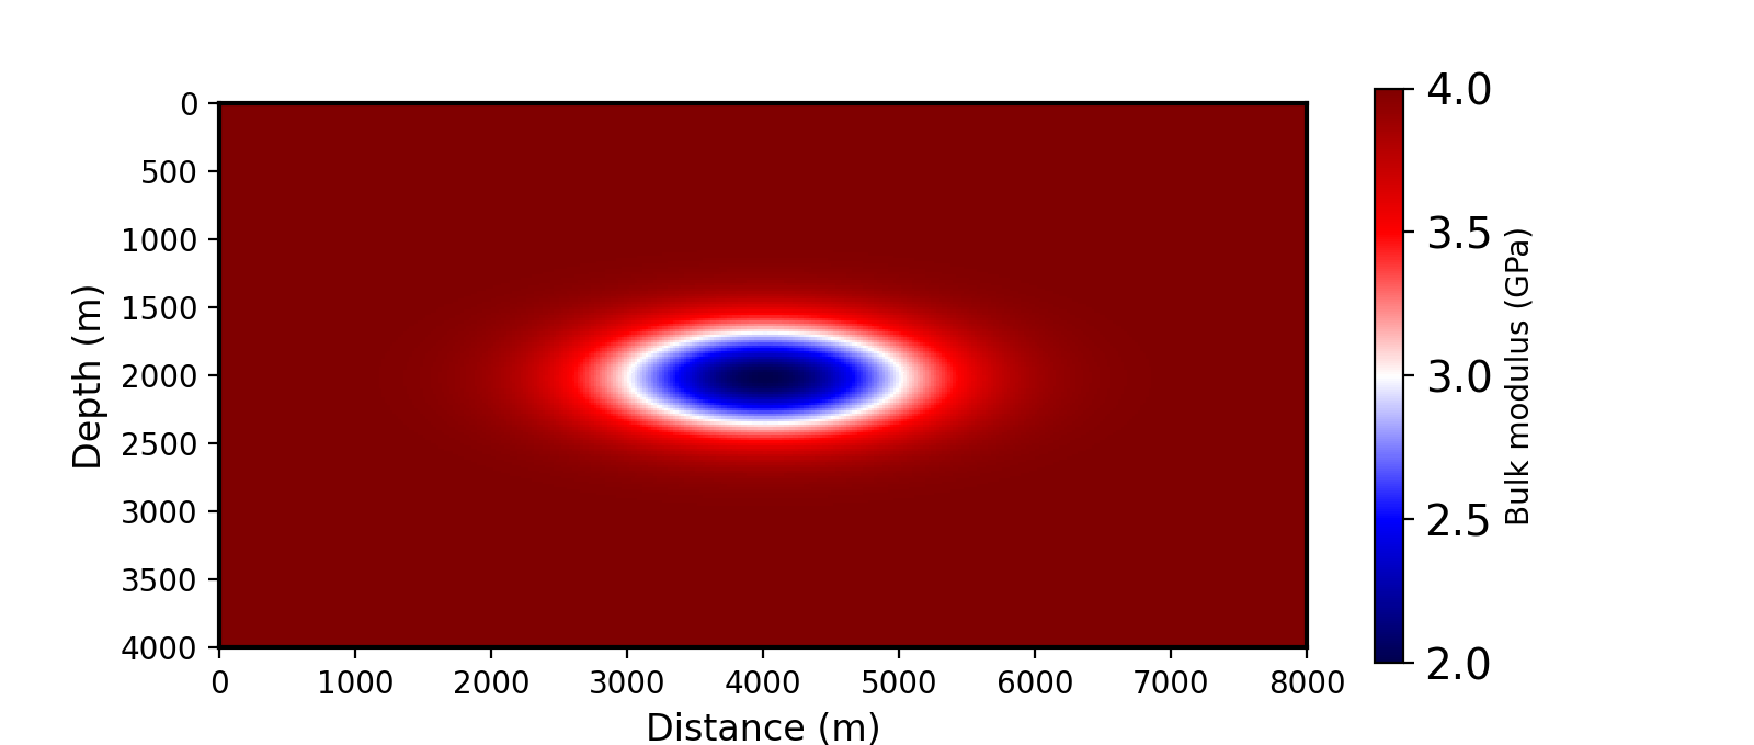
\includegraphics[width=0.40\textwidth]{dcwm}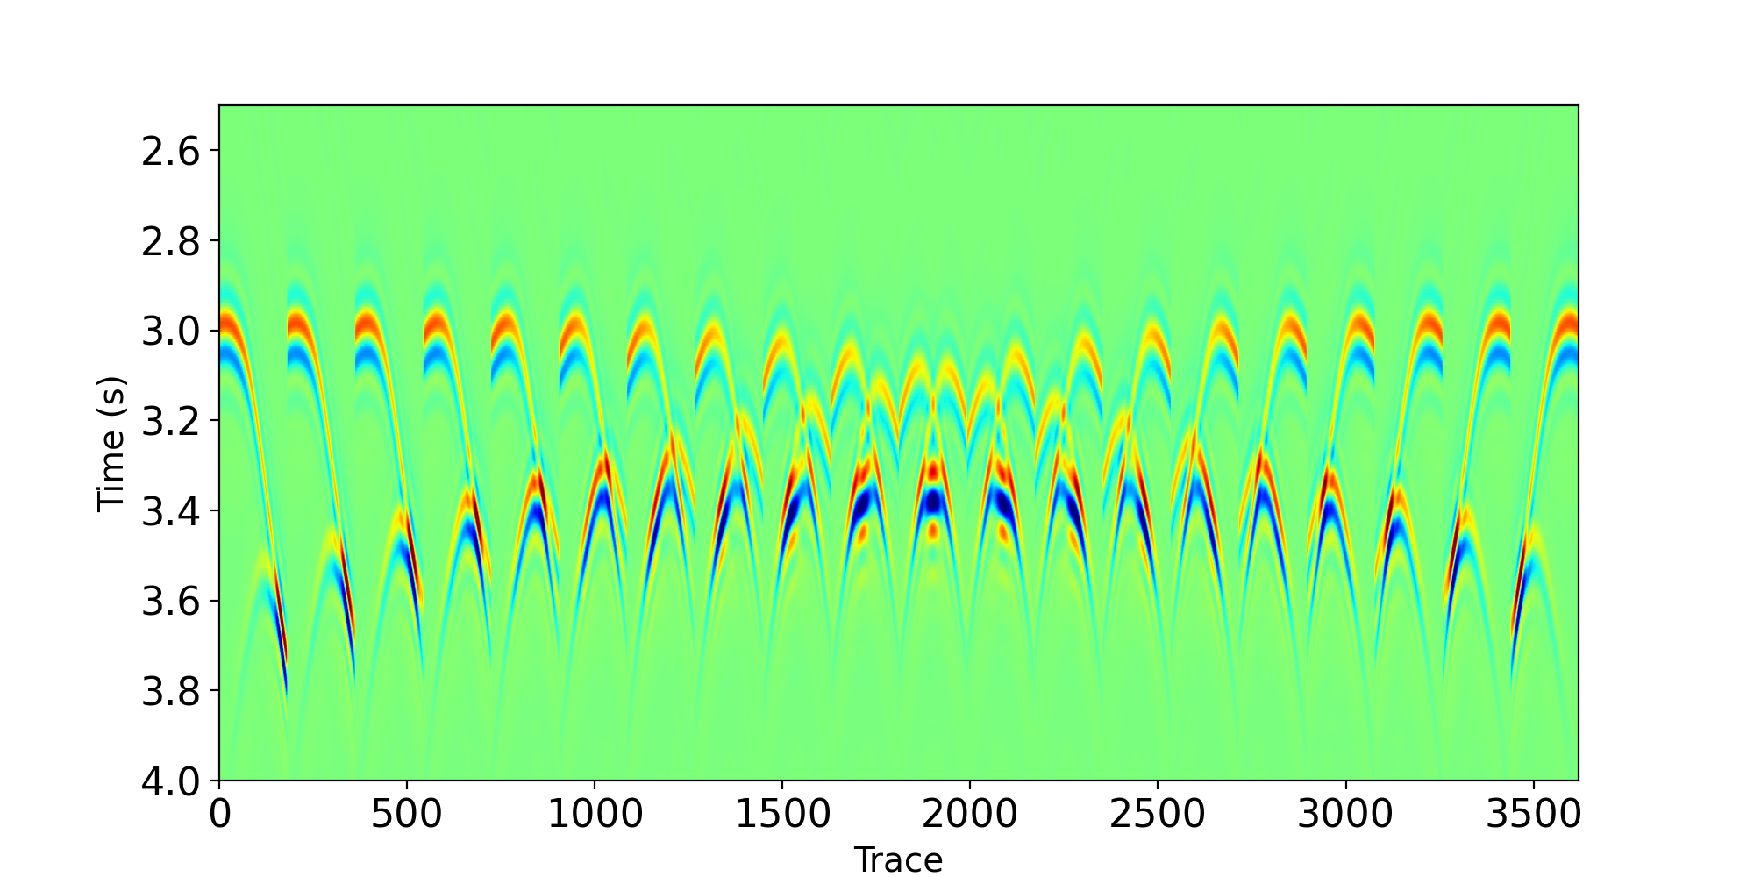
\includegraphics[width=0.40\textwidth]{dcwd20}
  \end{center}
  Left: extended ``lens''. Right: data traces, sources at $x_s=2000$
  m, receivers at
  $x_r=6000$ m.

  Interference between multiple waves (travel times) $\Rightarrow$ AWI
  behavies just like FWI (``cycle skips'') (S. '94, Huang 19, Pladys
  '21, Yong '23, S. '24)
}

\frame{
  ignore 2nd term, $d^* = p[\kappa^*] = 
  \rho a^*\partial_t f(t-\tau^*) +...$  ($a^*=a[\kappa^*]$ etc.)
  so 
  \[
    \us = \mbox{argmin}_u (\rho^2\|a \partial_tf * u(t-\tau) - a^*
    \partial_tf (t-\tau^*)\|^2 + \sigma\|u\|^2)
  \]
  \[
    = \frac{a^*}{a}g_{\sigma}(t-(\tau-\tau^*)),\, \hat{g}_{\sigma}(\omega) =
    \frac{\rho^2 a^2 \omega^2|\hat{f}(\omega)|^2}{\rho^2 a^2
      \omega^2|\hat{f}(\omega)|^2 + \sigma}
  \]
  whence
  \[
    J_{\rm AWI,\sigma} \approx \sum_{(\bx_r,\bx_s)\in X_{sr}}\left(
    (\tau-\tau^*)^2 + \frac{\|tg_{\sigma}\|^2}{\|g_{\sigma}\|^2} \right)
  \]
  Asymptotics: $f = \fl$ and $\sigma \propto \lambda$ then
  \[
    = \|\tau[\kappa]-\tau[\kappa]^*\|^2 + O(\lambda^2)
  \]
$O(\lambda^2)$ estimates for ``...'', other fine print - S. '24
  (arXiv) (related: Song '94)
  %Time error $\tau-\tau^*$ appears explicitly! (also $g_{\sigma}$ is even...)
 
}

%\frame{
%  so for each $(\bx_r,\bx_s) \in X_{sr}$,
%  \[
%    \|t\us\|^2 = \frac{(a^*)^2}{a^2}( (\tau-\tau^*)^2\|g_{\sigma}\|^2
%    + \|tg_{\sigma}\|^2 )
%  \]
%  \[
%    \|\us\|^2 = \frac{(a^*)^2}{a^2}\|g_{\sigma}\|^2
%  \]
  
%}
